\chapterauthor{Tim Warburton \& Ali Karakus}

\epigraph{I'm an egotistical bastard, and I name all my projects after myself. First Linux, now git.}{Linus Torvalds (caffeine aficionado)}

\minitoc

\section{A note on notation}

\noindent{\bf The text in a yellow box} is a set of commands that you can type into the terminal in your virtualbox. However, it is important that you understand that your present working directory is important for some commands. Where possible I have included change-directory (\verb|cd|) commands to make sure you are in the right directory to issue a command that is location sensitive. However you should start to pay attention to your present working directory by using the following command 
\myvbox[mytermbg]{pwd}
\noindent which will report the present working directory, i.e. where the terminal thinks your focus is in relative to the whole file system.

\vspace{8pt}\noindent {\bf Be alert when you see [SOME CAPITALIZED TEXT IN SQUARE BRACKETS]}: in the following there are several places where some part of the text for a Linux terminal command must be supplied by you. 

For instance a command that involves your VT NETID will require you to use substitute your actual NETID. When you see \texttt{[NETID]} in a yellow box command it means you should ignore the square brackets and replace NETID with your actual VT NETID. 

%In my case if I  see \texttt{cmda3634[NETID]} I will substitute \texttt{cmda3634tcew} since my VT NETID is tcew. 
Hopefully when you see \texttt{[SOME CAPITAL TEXT IN SQUARE BRACKETS]} it will be clear what text should be used in its place. Don't forget to lose the square brackets !

\section{Introduction}

Git is a distributed source code management system (\href{https://en.wikipedia.org/wiki/Git}{wiki}). Key things to know about Git: 
\begin{itemize}
    \item Git was created by Linus Torvalds to help with team development of his Linux project.
    \item It is becoming a standard mode for sharing and collaborating on coding projects.
    \item The word ``git'' is an english-ism for an unpleasant person and according to the Git wiki page Torvalds may have named Git after himself. Sigh.
    \item There are two parts to Git: a server that stores files for a project (repo or repository) and an app that interacts with the server to retrieve and possibly modify the files.
    \item More than one user can access and modify the contents of a repository if they have sufficient access rights. This allows multiple users to collaborate on a shared project.
\end{itemize}
In this class we will use \href{https://about.gitlab.com}{GitLab} online repository system to manage all course computer codes. In particular we will use the GitLab service provided by Virginia Tech and hosted at \href{https://code.vt.edu/}{https://code.vt.edu/} .  I have already set up a public repository where class example source code and other computer codes will be hosted. You can view this via the GitLab web interface: \href{https://code.vt.edu/tcew/cmda3634fa19}{https://code.vt.edu/tcew/cmda3634fa19}

\vspace{8pt}\noindent In the following we will discuss how to:

\begin{itemize}

    \item Create a private Git repository on the VT GitLab through the web interface.
    \item Install the Git command line application in your virtualbox.
    \item Create and add a secure shell key (ssh key) to your private Git repo.
    \item Clone the repository from the VT GitLab server onto your virtualbox.
    \item Navigate the local copy of your Git repo on your virtualbox's file system.
    \item Create and modify files in your local copy of the repo.
    \item Add your changes to the local repo via the Git command line application.
    \item Commit your changes to the local repo via the Git command line application.
    \item Push your changes from the local repo to the VT GitLab server.
\end{itemize}

\section{Creating your own private repository on the VT GitLab server}


The first step in creating a GitLab repository is to navigate in your browser to \href{https://code.vt.edu}{https://code.vt.edu} which is the online portal to the GitLab server that Virginia Tech maintains for the benefit of students, faculty, and staff. One special feature of this service is that it allows members of the VT community to create ``private'' repositories and choose who can access them. This feature is not typically included in the free services offered by GitHub \href{https://github.com/}{http://github.com} and BitBucket \href{https://bitbucket.org}{https://bitbucket.org}. Since your coursework must be submitted to a private repository we require that you use the GitLab repo hosted by VT. 

\begin{figure}[htbp!]
    \centering
    \fbox{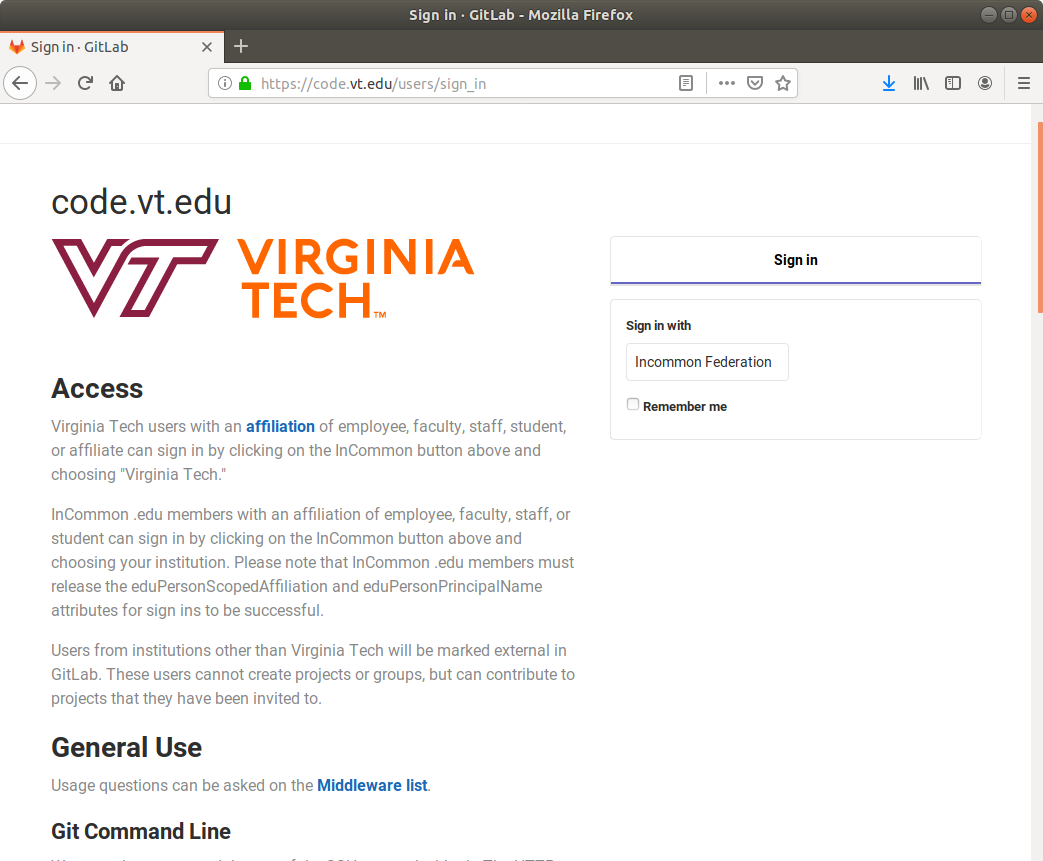
\includegraphics[width=0.66\textwidth]{figures/L03/signin_code_vt_edu.png}}
    \caption{Sign in page for \href{https://code.vt.edu}{https://code.vt.edu}. To access the VT GitLab service click on the cryptically labelled ``Incommon Federation'' button.}
    \label{signInCodeVtEdu.fig}
\end{figure}

When you access \href{https://code.vt.edu}{https://code.vt.edu} you will first click on the ``Incommon Federation'' button, type Virginia Tech in the dialog box, and then you will proceed to the VT two factor authentication system.  You will need to push a notification to your phone or other registered two factor device in order to gain access.


\begin{figure}[htbp!]
    \centering
    \fbox{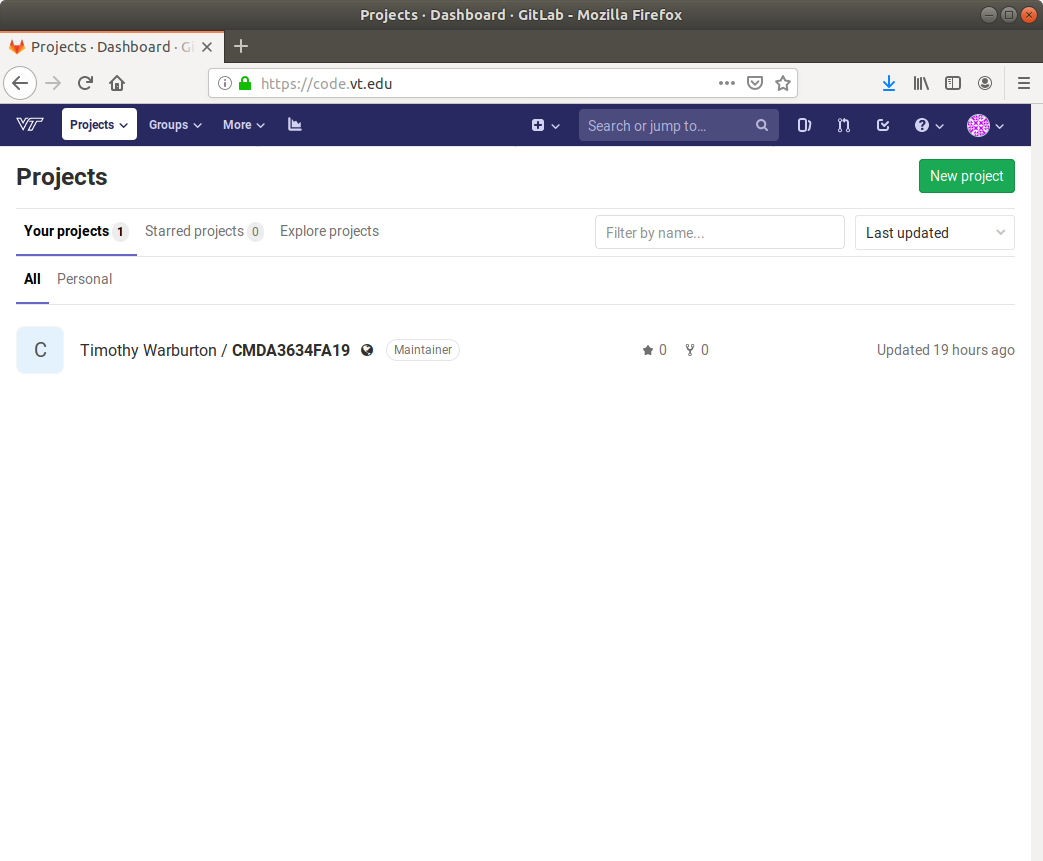
\includegraphics[width=0.66\textwidth]{figures/L03/account_code_vt_edu.png}}
    \caption{Project management page for \href{https://code.vt.edu}{https://code.vt.edu}. To create a new repository go ahead and click on the ``New Project'' button.}
    \label{projectsCodeVtEdu.fig}
\end{figure}

After completing this process you will land on your account page for the VT GitLab service. This is your portal for creating, modifying, and deleting your GitLab repositories. In Figure \ref{projectsCodeVtEdu.fig} you will see that I have already created a repository visible in the list of projects. Your Project will be empty unless you have previously created a repository on this site perhaps for a different class or project. 

\begin{figure}[htbp!]
    \centering
    \fbox{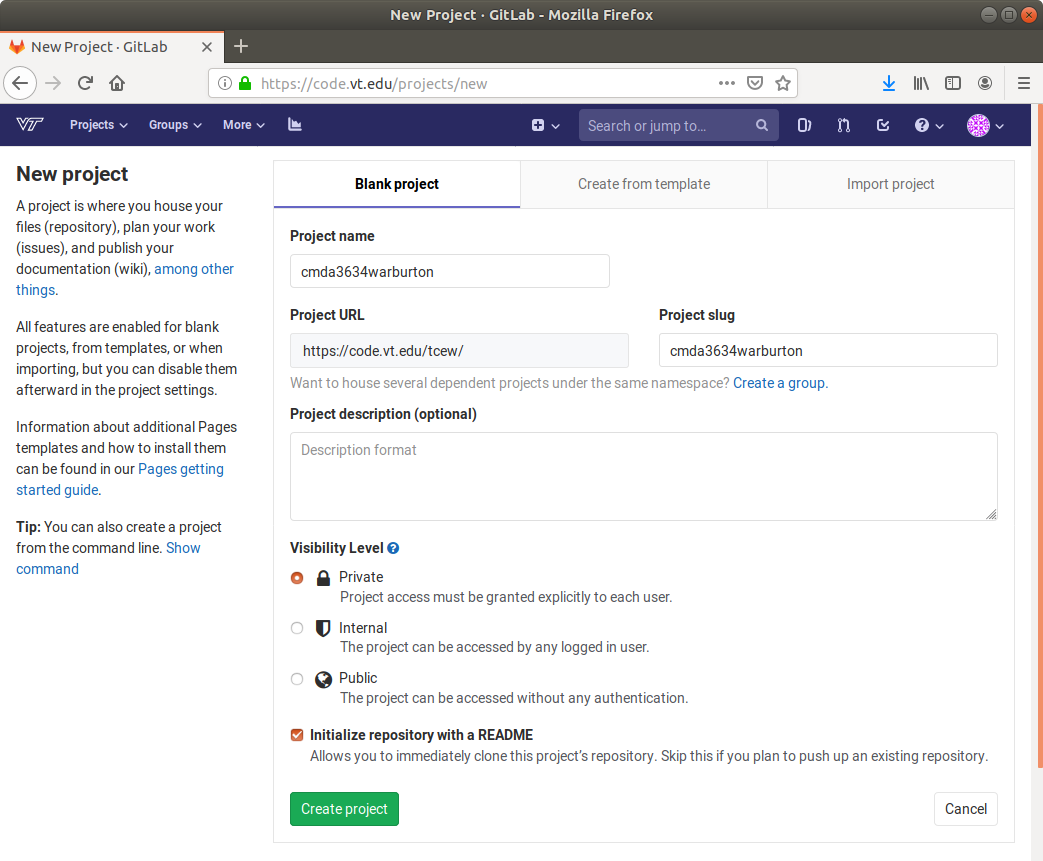
\includegraphics[width=0.45\textwidth]{figures/L03/correctedNewProject_code_vt_edu.png}}
      \fbox{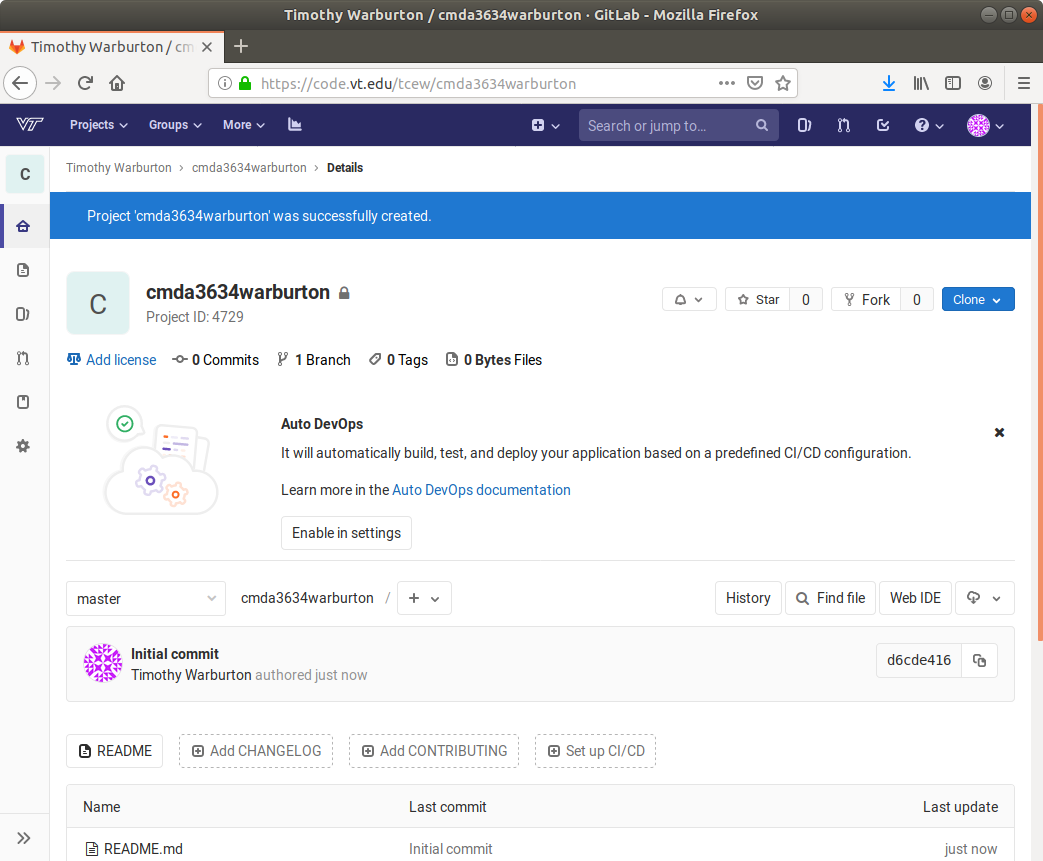
\includegraphics[width=0.45\textwidth]{figures/L03/afterNewProject_code_vt_edu.png}}
    \caption{Left: New Project creation page for \href{https://code.vt.edu}{https://code.vt.edu}. Go ahead and type in the cmda3634 for your project title, select ``Private'' and initialize a README. Right: after clicking ``Create Project''.}
    \label{newProjectCodeVtEdu.fig}
\end{figure}

To create a new GitLab repo click on the ``New Project'' button and follow instructions to create a private repository. You should name it:  cmda3634. Make sure that you specify it should be a ``Private'' repository and also click the ``Initialize repository with a README'' box.


\FloatBarrier


\newpage
\section{Installing the Git command line tool}

Since we will spend most of our time developing code from within the terminal command line it makes sense to interact with the Git app from the command line too. 

First things first, if you have not already done so start your virtualbox and launch a terminal. Next you can easily install the Git command line app using the \verb|apt-get| command:

\myvbox[mytermbg]{\# install the Git command line tool \\ \# using the apt-get command \\ \# which requires super user privilege provided by super-user-do (sudo) \\\\ sudo apt-get install git}

\vspace{8pt}\noindent {\bf Note}: useful tutorial on using \verb|apt-get| \href{https://codeburst.io/a-beginners-guide-to-using-apt-get-commands-in-linux-ubuntu-d5f102a56fc4}{here}.

\section{Creating an ssh key from your virtualbox terminal}

We first install the secure shell app with again using the VirtualBox terminal command line as follows

\myvbox[mytermbg]{\# install the secure shell command line tool \\ sudo apt-get install ssh}

\vspace{8pt}\noindent {\bf Note}: this will install the ssh app software in the virtualbox file system. i.e. once you have done this one time then you should not need to install it again. Later on in the course you will use the \verb|ssh| command line app to ``1ogin'' to a remote server in the VT Advanced Research Computing server room. For the moment we will just use it to create an ssh key that will let you access the private repo without constantly entering your password.

\vspace{8pt}\noindent In the following sequence of commands we use some of the commands from lecture 02 to 

\myvbox[mytermbg]{\# navigate to your home directory \\ cd \mytilde/ \\\\ \# make a hidden directory called .ssh \\ mkdir .ssh \\\\ \# navigate to the hidden .ssh directory \\ cd .ssh \\\\ \# use the ssh-keygen command line app to generate a public/private key pair \\ ssh-keygen -o  \\\\ \# check to see what got created using the ls command \\ ls -l }

You should see a list of commands, and in particular you should see \verb|id_rsa| and \verb|id_rsa.pub|. The private ssh key is given in text in the former, and the public key is given in the later file. Never reveal the contents of the \verb|id_rsa| private key to anyone. You can however copy the \verb|id_rsa.pub| to remote servers that you wish to access via ssh. Later in the semester you will copy that public key file to the ARC cluster to get password-free access.

\section{Adding an ssh key to your private repository on the VT GitLab server}

Now that you have generated your ssh public/private key pair you can use (only) the public key to set up password-free access to your private repo when you use the command line Git app. The first step is to reveal the public key using the \verb|cat| command

\myvbox[mytermbg]{\# inspect your ssh public key \\ cat \mytilde/.ssh/id\_rsa.pub}

The public key should now be visible in your terminal. The next step is a bit tricky: you need to enable copy-and-paste between the virtualbox Ubuntu guest OS and your regular operating system. Locate the virtualbox menu to enable bidirectional cut and paste and select it.
\begin{figure}[htbp!]
    \centering
    \fbox{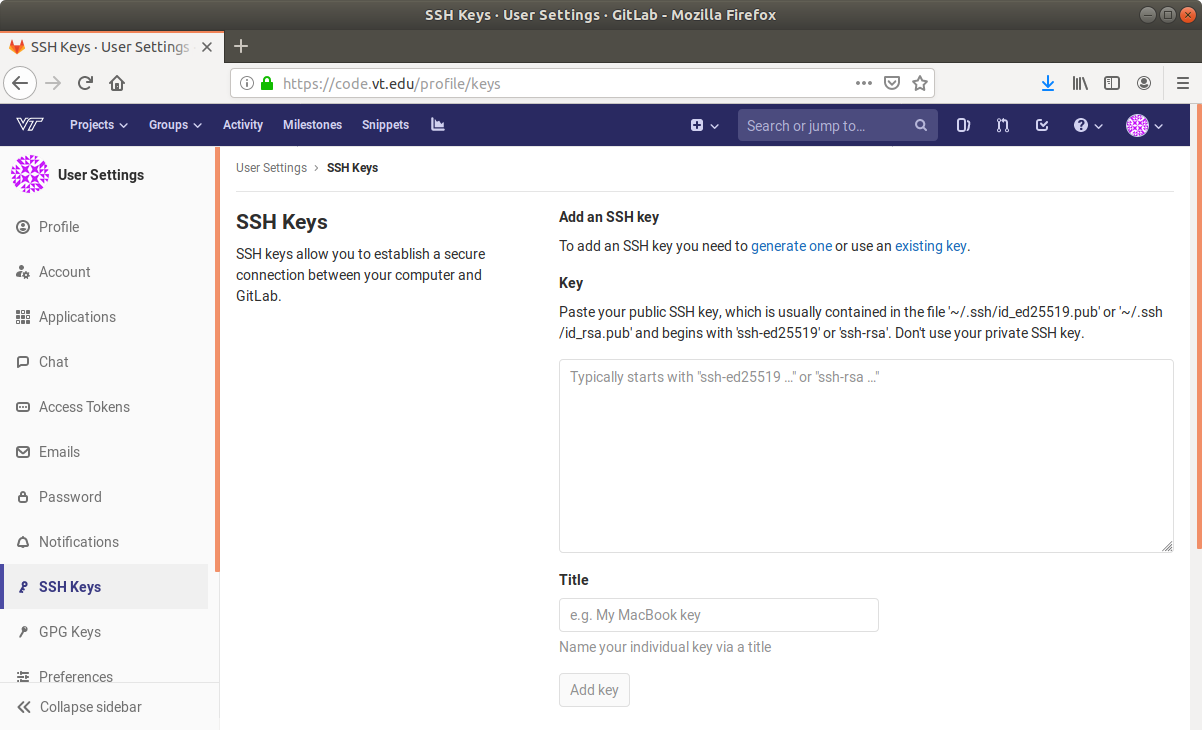
\includegraphics[width=0.8\textwidth]{figures/L03/sshKey_code_vt_edu.png}}
    \caption{Account settings for your VT GitLab account found at \href{https://code.vt.edu/profile/keys}{https://code.vt.edu/profile/keys}. Click on the SSH Keys button and then paste your ssh public key into the text rectangle under ssh key on the right hand side. }
    \label{sshKeyCodeVtEdu.fig}
\end{figure}
Now go ahead and copy the revealed ssh public key. Then navigate in your browser to \href{https://code.vt.edu/profile/keys}{https://code.vt.edu/profile/keys} select the SSH button on the left hand side and paste your ssh public key on the right hand side. See Figure \ref{sshKeyCodeVtEdu.fig} to confirm you are on the right track. 

When you have pasted your public key then choose a title for the key (say virtual box) and click the Add key button. If everything has gone well then you should be able to access the repo from your 


\section{Cloning the repo from the VT GitLab server to your virtualbox using the command line}

Now that we have set up the online repo and also set up password-free access it is time to ``clone'' the repository from the online server to your virtualbox. It is helpful to reflect on this for a few minutes. Right now the virtualbox running on your laptop is completely unaware of anything to do with the existence of the online repository or its contents. We need to use the Git command line tool \verb|git| to copy the contents of the online repository to the disk storage associated with the virtualbox on your laptop. To do this you should first create a directory where your local copy of the repo will reside, then use the \verb|git| command line app to clone the repo

\myvbox[mytermbg]{\# navigate to your home directory \\cd \mytilde/ \\\\ \# create a directory where your git repositories will live \\ mkdir class \\ mkdir class/git\\\\ \# navigate into new directory \\ cd class/git \\\\ \# clone the repo \\ \#(replace [NETID] with your VT netid \\  git clone git@code.vt.edu:[NETID]/cmda3634.git \\\\ \# check to see if repo was actually cloned \\ ls}

\noindent If the repo directory does not show up when you type \verb|ls| then seek help. Any number of things may have happened to prevent successful cloning.

\section{Navigating the local copy of your repo from the terminal command line}

The good news is that the local clone is really just a regular Linux directory with sub-directories. You can use the standard terminal commands to navigate within the clone. For instance
\myvbox[mytermbg]{cd \mytilde/class/git/cmda3634 \\ ls \\ mkdir L03 \\ cd L03 \\ emacs testFile.text }
\noindent When you save that file you will have made a new subdirectory that contains a text file. It is located within the directory structure of the local clone of the online repo. But it is important to recognise that although the file is contained within the directory structure, Git does not consider it part of the repository. 

You can query what Git thinks the status of the repo is with the following terminal command (assuming that your current working directory is located within the directory structure of the local clone)
\myvbox[mytermbg]{git status}
\noindent You should see that the \verb|testFile.text| is included on a list of ``Untracked files''. 

Go ahead and also check to see if the file shows up under the online interface by pointing your browser at \href{https://code.vt.edu/[NETID]/cmda3634}{https://code.vt.edu/[NETID]/cmda3634} where you replace NETID  with your own VT netid. That directory you created should not show up (at least not yet) since we need to explicitly add the file to the repo.

\section{Git Tutorials}

For additional tutorials see for instance the cheat sheets:
\begin{itemize}
    \item GitHub: \href{https://github.github.com/training-kit/downloads/github-git-cheat-sheet.pdf}{https://github.github.com/training-kit/downloads/github-git-cheat-sheet.pdf}. 
    \item BitBucket:
    \href{https://www.atlassian.com/git/tutorials/atlassian-git-cheatsheet}{https://www.atlassian.com/git/tutorials/atlassian-git-cheatsheet}
    \item GitLab: \href{https://about.gitlab.com/images/press/git-cheat-sheet.pdf}{https://about.gitlab.com/images/press/git-cheat-sheet.pdf}
    \item KeyCDN: \href{https://www.keycdn.com/blog/git-cheat-sheet}{https://www.keycdn.com/blog/git-cheat-sheet}
    \item Nina Jaeschke: \href{https://rogerdudler.github.io/git-guide/files/git_cheat_sheet.pdf}{https://rogerdudler.github.io/git-guide/files/git\_cheat\_sheet.pdf}
    \item {\bf Scott Chacon and Ben Straub's priceless text on working with Git}\\ \href{https://git-scm.com/book/en/v2}{https://git-scm.com/book/en/v2}.
\end{itemize}

You can also use your favorite search engine to find other tutorials on using Git. 

\section{Summary of Git commands so far}

In Table \ref{gitCommands.tab} we give a list of common use cases for the Git command line tool. 

\begin{table}[htbp!]
    \centering
    \begin{tabular}{l|l} \hline
      Action & \verb|git| commands \\ \hline
         Clone repo &  \texttt{git clone [URL OF REPO]}\\ \hline
         Add file change to local repo &  \texttt{git add [ FILE NAME]} \\
         Commit change to local repo & \texttt{git commit -m '[NOTE TO ATTACH TO COMMIT]'} \\
         Push committed changes to remote repo & \texttt{git push} \\ 
         Update local repo with remote changes & \texttt{git pull} \\ \hline
         Create a new branch & \texttt{git branch [NAME OF BRANCH TO CREATE]}\\
         Switch to a different branch & \texttt{git checkout [NAME OF BRANCH TO SWITCH TO]} \\ \hline
    \end{tabular}
    \caption{Summary of commonly used Git command line tool commands.}
    \label{gitCommands.tab}
\end{table}
\noindent In the next lecture we will  practice interacting with the online Git repo, present an overview of the branching structure of a git repository, and perhaps even try a merge. Review the cheat sheet prior to the lecture.
